\section{Comparative results}
\label{sec:comparative-results}

In this section the different algorithms designed for the metaheuristics will be compared to
the ILP model for a few different instances of the problem. But first, we will start by
briefly describing the instances used.

\subsection{Description of the instances used}
\label{sec:comparative-results:instances}

All the instances used to compare the different algorithms were purely randomly generated,
that is, there was not any change made by hand. There are two sets of different inputs: the
\textit{big} set of inputs and the inputs generated by one of the students of the course
\textit{********}, while the set of instances \textit{big} were generated by the author
of this report.

\hfill

Some of the inputs in the \textit{big} data set were generated following some rules: the
locations of all of the inputs were generated with some randomised space between them (as a
function of the parameter $D$) in order to ensure their feasibility for that matter, but only
the cities of all the inputs, but two of them, were generated with some randomised space
between them (as a function of $D$). This function is $\alpha D$, where $\alpha \in \mathbb{R}$
is a uniformly distributed random number in the interval $[0,1]$. All cities and locations
were generated within certain ranges of values of $x$ and $y$ and were different for almost
every input. The populations, working distances, installation costs, ..., were also randomly
generated within certain ranges, again different for most inputs. One particularity worth being
mentioned is that the capacities of the centres were generated slightly above the largest
population for all centres. On the one hand, this way of generating the instances does not
guarantee their feasibility, it only increases their chances to be so. On the other hand, this
does make the instances easy to solve: there is not much variety when it comes to the types of
centres used. However, they have been very useful to test the heuristics before switching to
bigger and more difficult instances.

\subsubsection{Optimal solutions and execution times}
\label{sec:comparative-results:instances:optimal-results}

In the following tables are presented the optimal values of the objective function of the ILP
formulation and the execution time needed to solve them. We also specify the number of cities,
locations and centre types.

\begin{table}[H]
    \centering
    \noindent
    \begin{tabular}{cccccc}
        \toprule
        Instance name & \# Locations & \# Cities & \# Centre types & ILP & Time (s) \\
        
        \midrule
        
        $big-16$    & 32    & 14    & 3     & 1892.960     &   1.482 \\
        $big-17$    & 37    & 11    & 2     & 1354.040     &   3.182 \\
        $big-20$    & 49    & 11    & 3     &  536.200     &   2.095 \\
        $big-21$    & 42    & 21    & 8     &  582.132     &   2.532 \\
        $big-23$    & 31    & 18    & 8     &  127.876     &   1.724 \\
        $big-24$    & 40    & 23    & 6     & 3607.100     &  19.440 \\
        $big-25$    & 47    & 19    & 8     &  319.376     &   2.527 \\
        $big-26$    & 44    & 25    & 14    &  487.323     &   3.524 \\
        $big-29$    & 46    & 26    & 11    &  695.350     &   4.240 \\
        $big-30$    & 37    & 30    & 13    & 1655.110     &   3.660 \\
        
        \midrule
        
        $t-5$       & 22    & 50    & 18    & 88350.300    & 347.768 \\
        $t-6$       & 22    & 50    & 18    & 52254.000    &   4.305 \\
        
        \bottomrule
    \end{tabular}
    \centeredcaption{Size, optimal solution and time to reach it for each instance.}
    \label{table:instances}
\end{table}

The inputs \textit{t}-$\{5,6\}$ are the only instances by \textit{********} that will be
used in this project.

\subsection{Local Search}
\label{sec:comparative-results:local-search}

The local search procedure consists on two parts: the greedy construction algorithm and the
neighbourhood exploration, explained in section \ref{sec:metaheuristics:greedy-algorithms}.
In the first place, after performing some experiments with instances of several sizes and
difficulty, it seems that this construction procedure is good enough to reach optimality for
those that are small, but not so much as soon as the size of the instance increases. However,
this procedure is startlingly fast, a highly desirable feature for these kind of procedures.

\hfill

Now, the neighbourhood exploration algorithm, in spite of always using the \textit{Best}
policy, does not produce the results we were expecting, that is, results close to the optimum
solution. This is due to two main reasons: this procedure, when applied to solutions greedily
constructed, does not improve them too much since locations already have the cheapest centres
that can be installed hence making it impossible to either remove or replace them. The
other reason is that, in spite of actually being capable of improving some instances, the
speed at which this algorithm converges is too fast, that is, this algorithm finds very soon a
dead-end in the feasible neighbourhood space, even when applied to randomly constructed
instances (see section \ref{sec:comparative-results:grasp}). Therefore, this procedure is made
to stop when no improvement is made or when a maximum of iterations is reached.

\hfill

See, for instance, the following tables, where is presented the performance of this procedure
for several \textit{big} inputs:

\begin{table}[H]
    \centering
    \noindent
    \begin{tabular}{cccccc}
        \toprule
        Instance name & Time (s) & Objective Function & Gap & Iteration &
        \# Neighbours explored \\
        
        \midrule
        
        $big-16$    & 0.000    & 2832.776   & 939.816 & 0     & 0     \\
                    & 0.000    & 2517.283   & 624.323 & 1     & 1     \\
        
        \midrule
        
        $big-17$    & 0.000    & 1943.056   & 589.016 & 0     & 0     \\
        
        \midrule
        
        $big-20$    & 0.000    &  612.800   &  76.600 & 0     &  0     \\
                    & 0.000    &  536.200   &   0.000 & 1     &  1     \\
        
        \midrule
        
        $big-25$    & 0.000    &  479.064   & 159.688 & 0     &  0     \\
                    & 0.000    &  439.142   & 119.766 & 1     &  6     \\
                    & 0.000    &  399.220   &  79.844 & 2     &  4     \\
        
        \midrule
        
        $big-30$    & 0.000    & 2373.196   & 718.086 & 0     &  0     \\
                    & 0.000    & 2137.012   & 481.902 & 1     &  4     \\
                    & 0.000    & 2026.671   & 371.561 & 2     &  3     \\
                    & 0.000    & 1916.330   & 261.220 & 3     &  1     \\
        
        \bottomrule
    \end{tabular}
    \centeredcaption{Traces extracted from the execution of the local search procedure. The
    \textit{Gap} values represent the difference in absolute value between the optimal
    solution and the solution found using Local Search.}
    \label{table:local-search:traces}
\end{table}

Notice how the previous description of these algorithms fits the data presented in table
\ref{table:local-search:traces}: there is a fast convergence of the algorithm (very few
iterations until no improvement is made) and the size of the neighbourhood set is significantly
small. In only one of the chosen inputs the optimal solution is reached (instance
\textit{big-20}). Moreover, there is one instance where the neighbourhood exploration does not
produce any result (instance \textit{big-17}).

\hfill

Just to confirm what already seems to be true enough, in the following two figures is presented
the same information for the instances \textit{t-5} and \textit{t-6}. In blue we find the
value of the objective function obtained by the local search procedure in iterations $1,2,...$.
In the iteration 0 the value corresponds to the solution constructed with the greedy
constructor. This is bottomed by a red line with the value of the optimal solution. The
dotted line represents the number of neighbours explored. The execution time is always 0.

\begin{figure}[H]
    \centering
    \begin{subfigure}{0.45\textwidth}
        \centering
        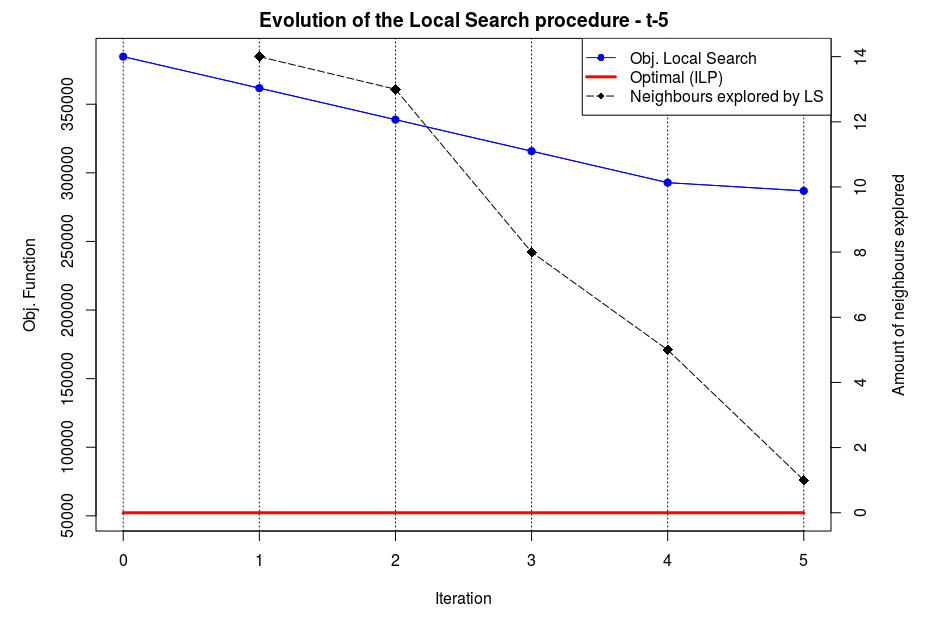
\includegraphics[scale=0.275]{metaheuristics/LS-miquel-tubau-5}
        \centeredcaption{Illustration of the trace for the input \textit{t-5}.}
        \label{fig:local-search:traces:t-5}
    \end{subfigure}
    \begin{subfigure}{0.45\textwidth}
        \centering
        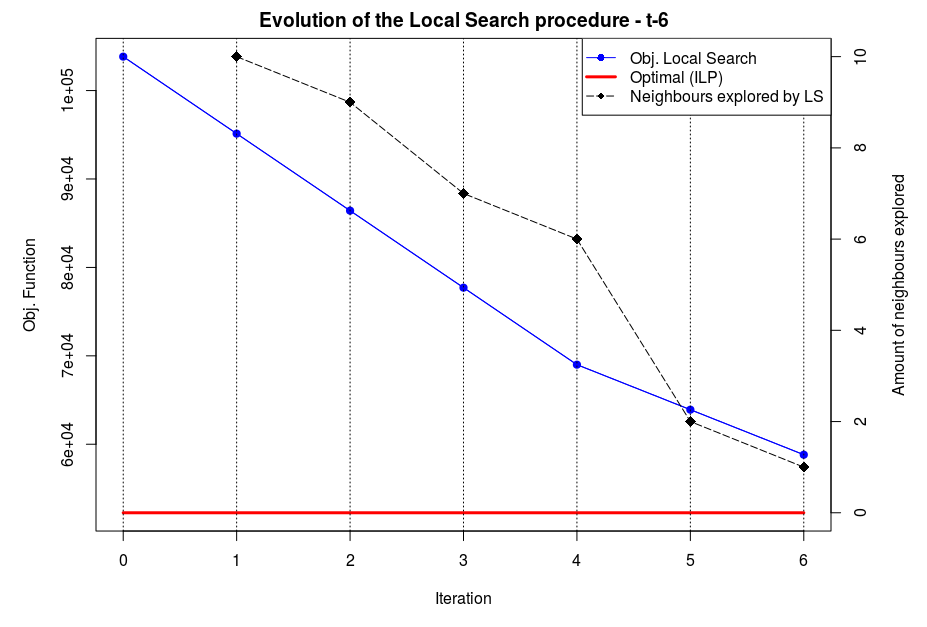
\includegraphics[scale=0.275]{metaheuristics/LS-miquel-tubau-6}
        \centeredcaption{Illustration of the trace for the input \textit{t-6}.}
        \label{fig:local-search:traces:t-6}
    \end{subfigure}
    \centeredcaption{Two traces of the Local Search procedure.}
    \label{fig:local-search:traces}
\end{figure}

Notice that the total amount of neighbours explored is greater when we use input \textit{t-5},
another aspect of that input that may be used to explain its difficulty along with the big
amount of time taken by the ILP solver.

\hfill

For all the executions the policy of the neighbourhood exploration algorithm was 
\textit{Best-Improvement}.

\subsection{GRASP}
\label{sec:comparative-results:grasp}

The GRASP procedure is a simple procedure that, in general terms, constructs an instance
randomly, improves it by using, in this case, a local search procedure, and is executed for a
fixed number of iterations. The method described in section
\ref{sec:metaheuristics:randomised-construction} for randomly constructing a solution poses a
serious problem when it comes to generate a feasible instance: there is absolutely no guarantee
that it is always feasible. When this happens, the method will skip that iteration and try to
generate a feasible solution.

\hfill

In figure \ref{fig:trace:grasp:t-5-simple} we see a short execution of the GRASP procedure:

\begin{figure}[H]
    \centering
    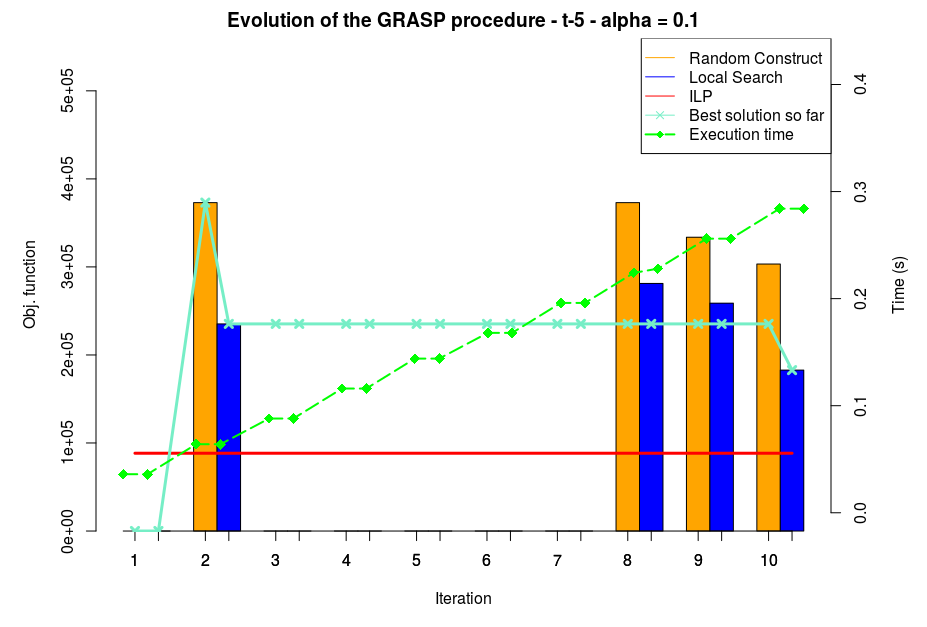
\includegraphics[scale=0.375]{metaheuristics/GRASP-miquel-tubau-5--0-1-simple}
    \centeredcaption{Illustration of the trace for the input \textit{t-5}, $\alpha = 0.1$.}
    \label{fig:trace:grasp:t-5-simple}
\end{figure}

In this figure we find all relevant information we need to know to explain the main
features, in the short term, of this procedure. In orange we find the value of the solutions
obtained by the random constructor and in blue the value of the solution improved by the local
search procedure for 10 iterations. In light blue we find the value of the best solution found
until the specified iteration. The red line represents again the value of the optimal solution
found by the ILP model, and in green the execution time.

\hfill

First and foremost, as anyone could notice, there are missing values for some of the
iterations. That means that the random constructor produced an infeasible solution. However,
the time does not stop and continues growing. But it does so linearly, a highly desirable
property for this procedure. This simple graph illustrates the complete behaviour of this
procedure. While there are some iterations that do not produce a better solution, or no
solution at all, the method always keeps the best solution, the value of which is represented
in the light-blue line.

\hfill

Now, this method, although designed to provide many different solutions by randomly
constructing them and improving them later on, does not work the same way for all instances,
and for some of them it is clearly useless. Take, for instance, inputs \textit{big-24} and
\textit{big-25}. The evolution of this procedure for different values of $\alpha$ shows that,
even after waiting for three times as much time as it takes the ILP solver to find the optimum,
reaching the optimum is nearly impossible. The figures showing this evolution are the
following:

\hfill

\begin{figure}[H]
    \centering
    \begin{subfigure}{0.45\textwidth}
        \centering
        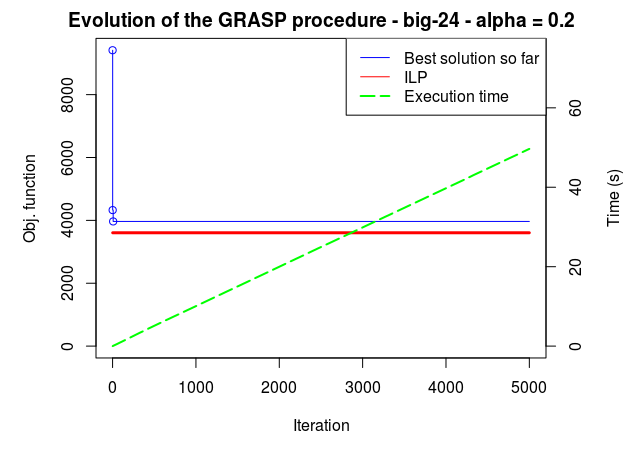
\includegraphics[scale=0.275]{metaheuristics/GRASP-big-instance-24--0-2}
        \centeredcaption{Illustration of the trace for the input \textit{big-24},
        $\alpha = 0.2$. Best objective = $3967.81$.}
        \label{fig:trace:grasp:big-24:0.2}
    \end{subfigure}
    \begin{subfigure}{0.45\textwidth}
        \centering
        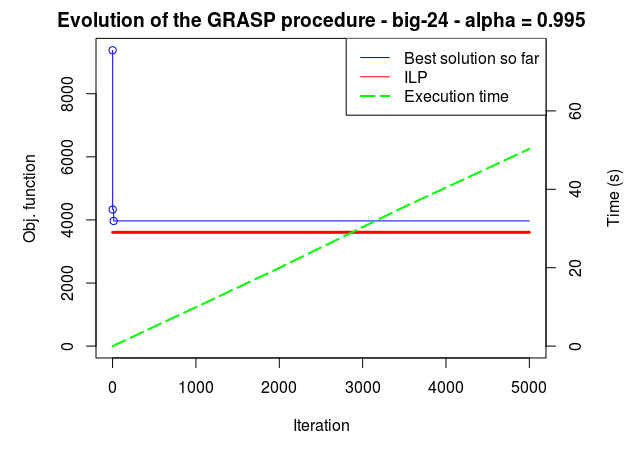
\includegraphics[scale=0.275]{metaheuristics/GRASP-big-instance-24--0-995}
        \centeredcaption{Illustration of the trace for the input \textit{big-24},
        $\alpha = 0.995$. Best objective = $3967.81$.}
        \label{fig:trace:grasp:big-24:0.995}
    \end{subfigure}
    \begin{subfigure}{0.45\textwidth}
        \centering
        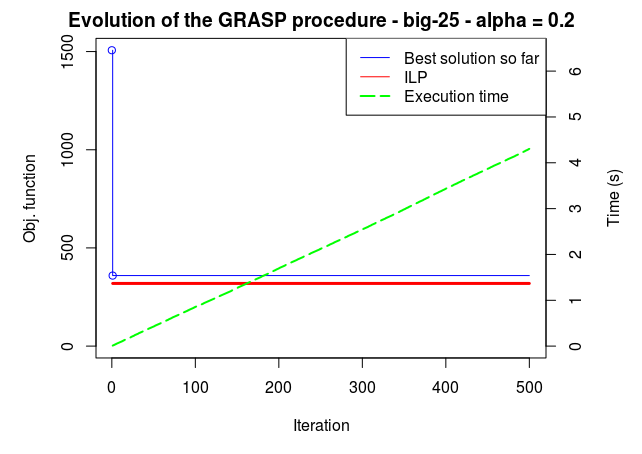
\includegraphics[scale=0.275]{metaheuristics/GRASP-big-instance-25--0-2}
        \centeredcaption{Illustration of the trace for the input \textit{big-25},
        $\alpha = 0.2$. Best objective = $359.298$.}
        \label{fig:trace:grasp:big-25:0.2}
    \end{subfigure}
    \begin{subfigure}{0.45\textwidth}
        \centering
        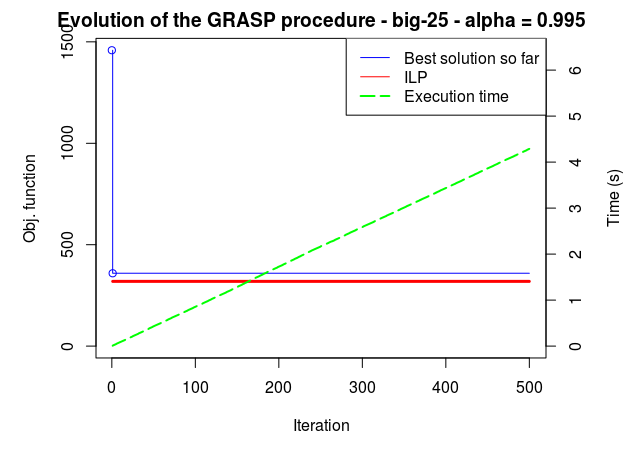
\includegraphics[scale=0.275]{metaheuristics/GRASP-big-instance-25--0-995}
        \centeredcaption{Illustration of the trace for the input \textit{big-25},
        $\alpha = 0.995$. Best objective = $359.298$.}
        \label{fig:trace:grasp:big-25:0.995}
    \end{subfigure}
    \centeredcaption{Traces of the GRASP procedure for two inputs and different values of
    $\alpha$.}
    \label{fig:trace:grasp:bigs}
\end{figure}

\hfill

Obviously, this procedure's quality highly depends on the quality of the random constructor
and the neighbourhood exploration. These two do not seem to work well with the previous
instances due to their low difficulty and size. Although the optimum is never reached in these
cases, and the evolution is quite poor, the time increases linearly, something that was already
expected when inspecting the behaviour in figure \ref{fig:trace:grasp:t-5-simple}. And indeed,
the difficulty affects the behaviour of the procedure. See the following figures where we try
to solve the instances \textit{t-5} and \textit{t-6}.

\begin{figure}[H]
    \centering
    \begin{subfigure}{0.45\textwidth}
        \centering
        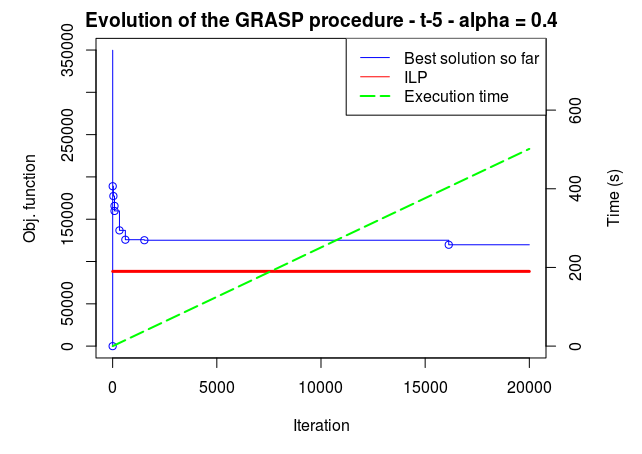
\includegraphics[scale=0.275]{metaheuristics/GRASP-miquel-tubau-5--0-4}
        \centeredcaption{Illustration of the trace for the input \textit{t-5},
        $\alpha = 0.4$. Best objective = $119848$.}
        \label{fig:trace:grasp:t-5:0.4}
    \end{subfigure}
    \begin{subfigure}{0.45\textwidth}
        \centering
        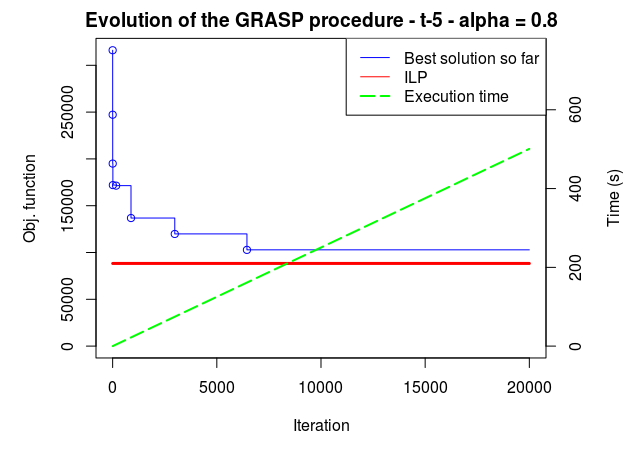
\includegraphics[scale=0.275]{metaheuristics/GRASP-miquel-tubau-5--0-8}
        \centeredcaption{Illustration of the trace for the input \textit{t-5},
        $\alpha = 0.8$. Best objective = $102851$.}
        \label{fig:trace:grasp:t-5:0.8}
    \end{subfigure}
    \begin{subfigure}{0.45\textwidth}
        \centering
        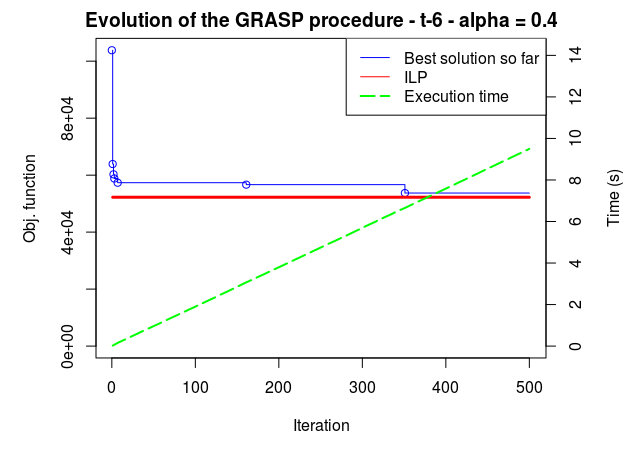
\includegraphics[scale=0.275]{metaheuristics/GRASP-miquel-tubau-6--0-4}
        \centeredcaption{Illustration of the trace for the input \textit{t-6},
        $\alpha = 0.4$. Best objective = $53727$.}
        \label{fig:trace:grasp:t-6:0.4}
    \end{subfigure}
    \begin{subfigure}{0.45\textwidth}
        \centering
        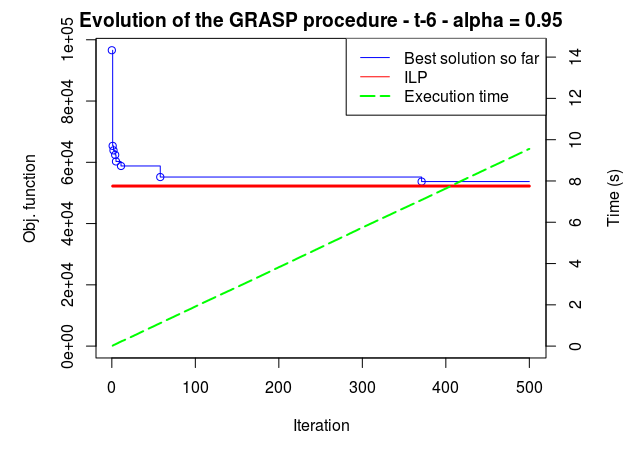
\includegraphics[scale=0.275]{metaheuristics/GRASP-miquel-tubau-6--0-95}
        \centeredcaption{Illustration of the trace for the input \textit{t-6},
        $\alpha = 0.95$. Best objective = $53727$.}
        \label{fig:trace:grasp:t-6:0.95}
    \end{subfigure}
    \centeredcaption{Evolution of the GRASP procedure for inputs \textit{t-5} and \textit{t-6}
    and different values of $\alpha$.}
    \label{fig:trace:grasp:ts}
\end{figure}

With these figures we see that the procedure improves the solution slightly over time. This
means that there may be hope to improve the solution even more if we waited enough time.
However, in figures \ref{fig:trace:grasp:t-5:0.4} and \ref{fig:trace:grasp:t-5:0.8} the
procedure already took as much time as the ILP solver (actually, slightly more), and in figures
\ref{fig:trace:grasp:t-6:0.4} and \ref{fig:trace:grasp:t-6:0.95} the procedure took twice as
much time as the ILP solver. Besides, there is no improvement at all in the solutions for
thousands of iterations in the first pair, and hundreds of iterations in the second. Thus, the
procedures proposed in section \ref{sec:metaheuristics:randomised-construction} are not good
enough to solve these instances.

\hfill

Notice another two aspects, though, that are that the parameter $\alpha$ neither seems to have
much effect on the execution time or on the quality of the best solution found at the end of
the execution, for the same number of iterations.

\subsection{BRKGA}
\label{sec:comparative-results:brkga}

This is the last procedure that will be commented in this report. In section
\ref{sec:metaheuristics:chromosome-decoder} is explained how the BRKGA procedure depends on a
chromosome decoder. In this section is evaluated the impact of this decoder and the BRKGA's
parameters on the quality of the solutions found. To do that, we will follow the
recommendations given in the article \cite{brkga} for the choice of the parameters.

\hfill

We applied three different values for the total size of the population defined as a function
of the parameter $a \in \mathbb{N}$: $p = a \cdot n$, where $n$ is the size of the chromosome,
which, according to the description of the decoder, is the amount of cities for each instance.
See table \ref{table:instances} in section
\ref{sec:comparative-results:instances:optimal-results} to see the description of each
instance. With this parameter set, the others were defined as $p_e = 0.175p$, $p_m = 0.2p$,
and then four different values for the probability of inheritance were tried to have more
diversity in results of experimentation $\rho_e = 0.5, 0.6, 0.7, 0.8$.

\hfill

The figures presented have a common format: in four different colours are presented the
values of the best solution at every generation of the population, one for each value of
$\rho_e$. The value of the parameter $a$ is specified at the top of each figure. The values
of $p$, $p_e$ and $p_m$ are are also specified, but in the caption, and in a dotted red line
is denoted the value of the optimal solution found with the ILP solver. The other coloured
and dotted lines correspond to the execution time in seconds of the procedure. Their
corresponding axis is found to the right of the figures.

\hfill

The first results recorded are very disappointing. These are the results of this procedure
when applied to the instances \textit{big-24} and \textit{big-25}. We can see in figure
\ref{fig:trace:brkga:big-24--big-25} how the values of the best solution found throughout the
hundreds of generations do not improve a bit (with just one exception) for any value of
$\rho_e$ and $a$ and do not seem to be willing to get close to the optimal value (in red).
This happened in a time that is a few times larger than the ILP needed to solve the instance,
therefore we should not expect the results to improve much more with the chosen configuration
of parameters.

\begin{figure}[H]
    \centering
    \begin{subfigure}{0.45\textwidth}
        \centering
        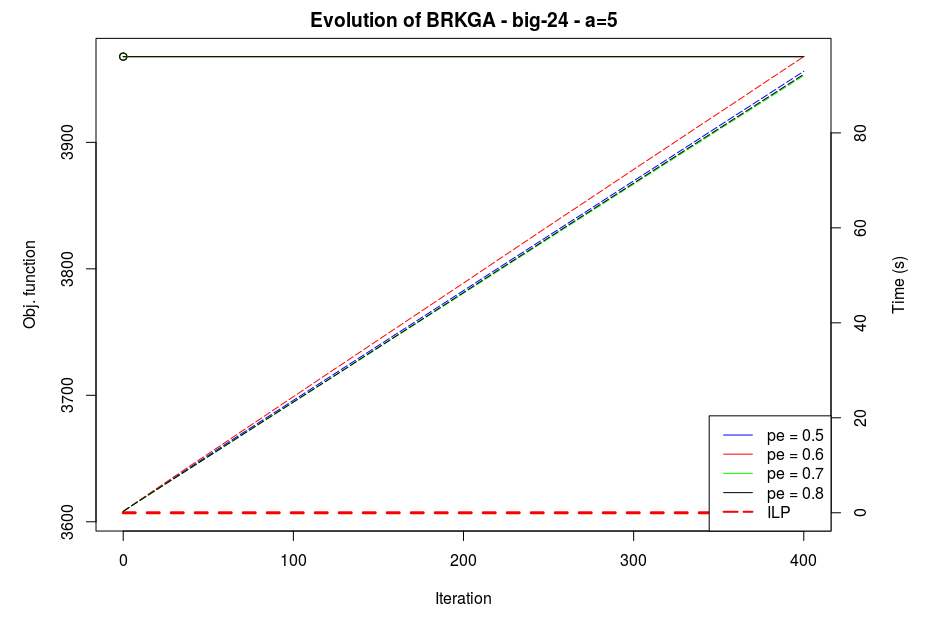
\includegraphics[scale=0.245]{metaheuristics/BRKGA-big-instance-24--5}
        \centeredcaption{Illustration of the trace for the input \textit{big-24}.
        $a = 5$, $p=115$, $p_e=20$, $p_m=23$.}
        \label{fig:trace:brkga:big-24:5}
    \end{subfigure}
    \begin{subfigure}{0.45\textwidth}
        \centering
        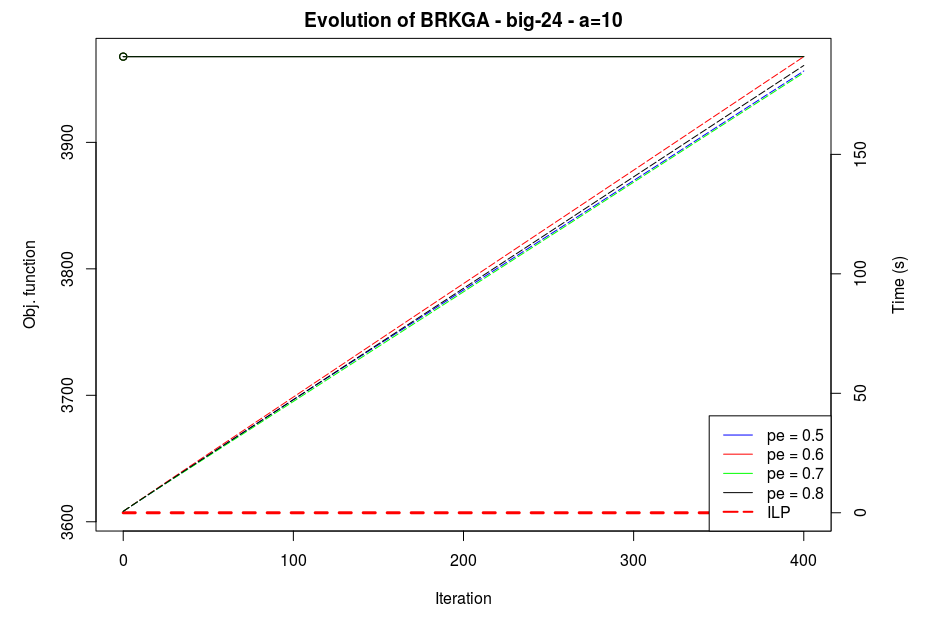
\includegraphics[scale=0.245]{metaheuristics/BRKGA-big-instance-24--10}
        \centeredcaption{Illustration of the trace for the input \textit{big-24}.
        $a = 10$, $p=230$, $p_e=40$, $p_m=46$.}
        \label{fig:trace:brkga:big-24:10}
    \end{subfigure}
    \begin{subfigure}{0.45\textwidth}
        \centering
        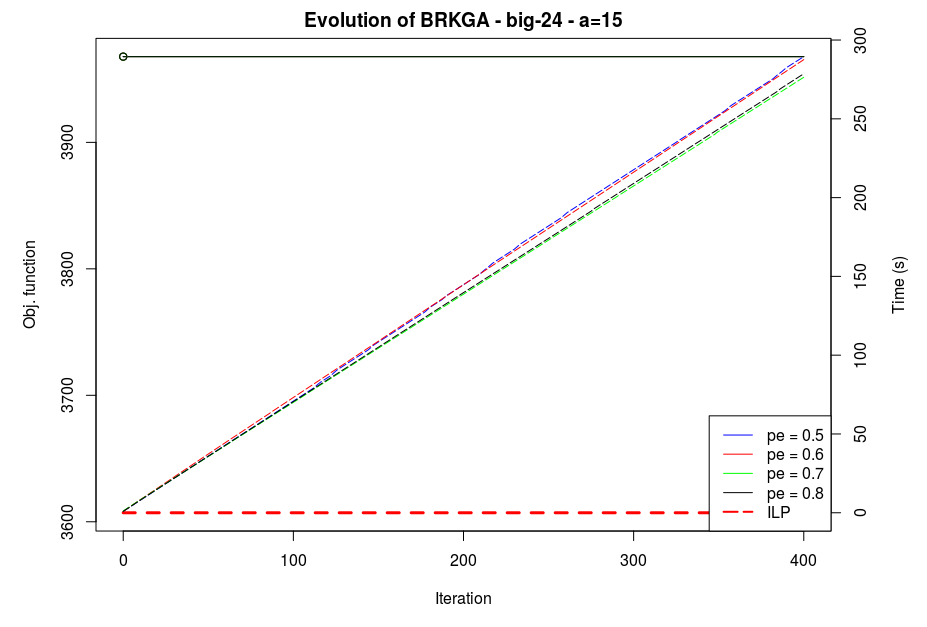
\includegraphics[scale=0.245]{metaheuristics/BRKGA-big-instance-24--15}
        \centeredcaption{Illustration of the trace for the input \textit{big-24}.
        $a = 15$, $p=345$, $p_e=60$, $p_m=69$.}
        \label{fig:trace:brkga:big-24:15}
    \end{subfigure}
    \begin{subfigure}{0.45\textwidth}
        \centering
        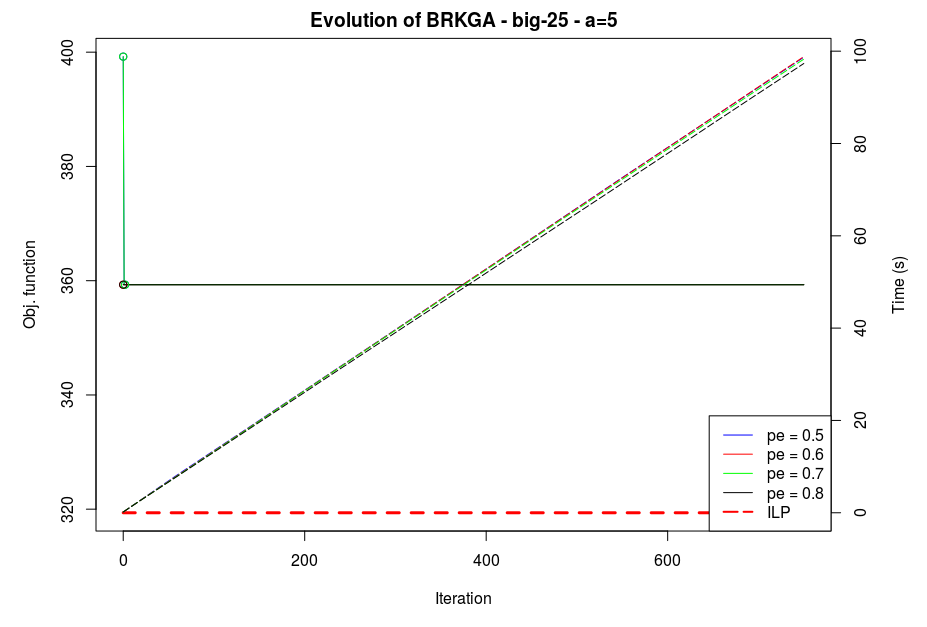
\includegraphics[scale=0.245]{metaheuristics/BRKGA-big-instance-25--5}
        \centeredcaption{Illustration of the trace for the input \textit{big-25}.
        $a = 5$, $p=95$, $p_e=16$, $p_m=19$.}
        \label{fig:trace:brkga:big-25:5}
    \end{subfigure}
    \begin{subfigure}{0.45\textwidth}
        \centering
        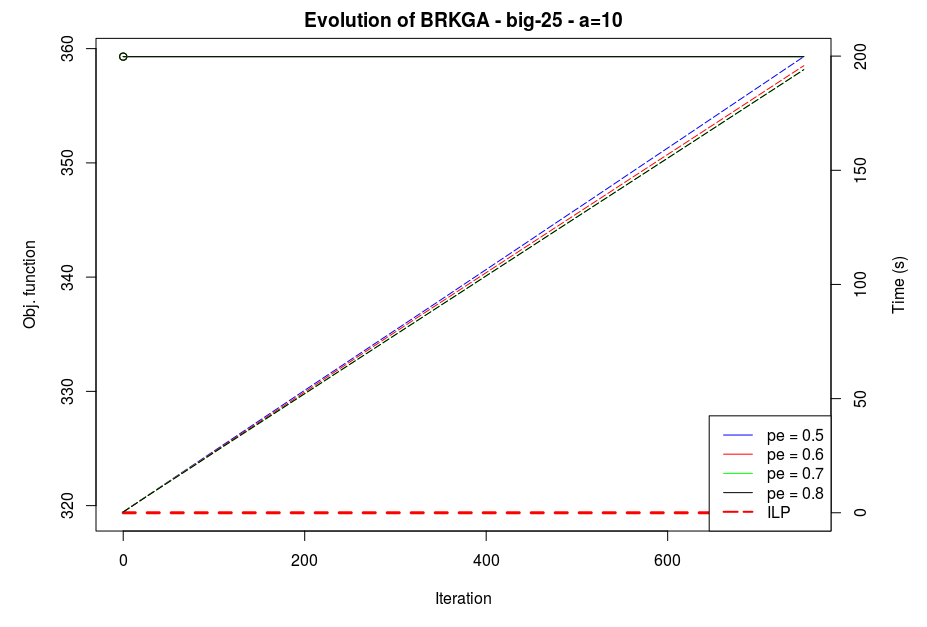
\includegraphics[scale=0.245]{metaheuristics/BRKGA-big-instance-25--10}
        \centeredcaption{Illustration of the trace for the input \textit{big-25}.
        $a = 10$, $p=190$, $p_e=33$, $p_m=38$.}
        \label{fig:trace:brkga:big-25:10}
    \end{subfigure}
    \begin{subfigure}{0.45\textwidth}
        \centering
        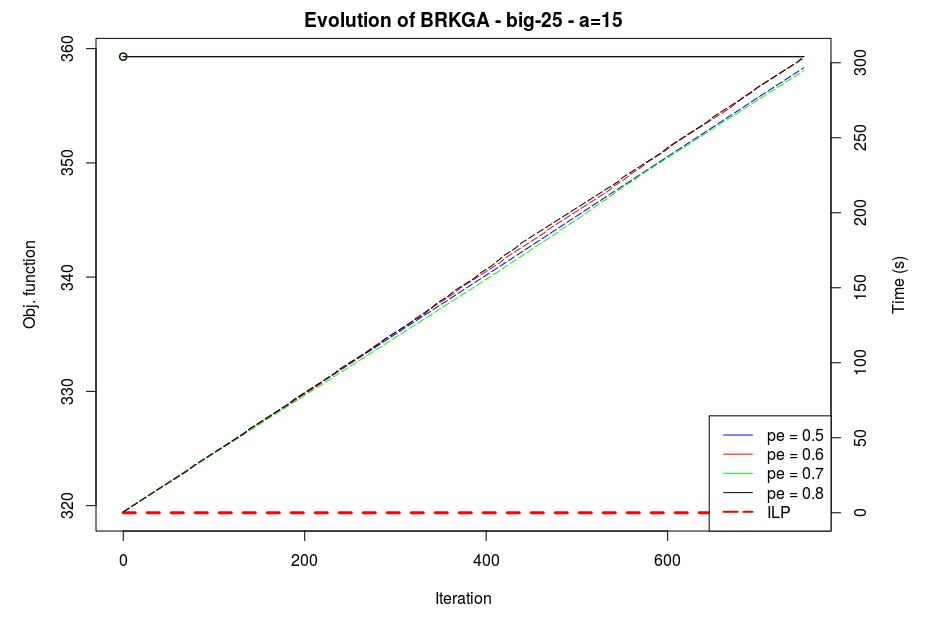
\includegraphics[scale=0.245]{metaheuristics/BRKGA-big-instance-25--15}
        \centeredcaption{Illustration of the trace for the input \textit{big-25}.
        $a = 15$, $p=285$, $p_e=49$, $p_m=57$.}
        \label{fig:trace:brkga:big-25:15}
    \end{subfigure}
    \centeredcaption{Evolution of the BRKGA procedure for the inputs \textit{big-24} and
    \textit{big-25} and values of $a = 5, 10, 15$.}
    \label{fig:trace:brkga:big-24--big-25}
\end{figure}

However, the results were more promising with the inputs \textit{t-5} and \textit{t-6} where
the difficulty of the instances is greater. We can see in figure \ref{fig:trace:brkga:t-5--t-6}
the impact in the behaviour on the procedure the parameters $p$, $p_e$, $p_m$ and $\rho_e$
have. In contrast with the previous instances, we can see how by increasing the value of
$\rho_e$ the value of the best solution improves bit by bit over time. Unfortunately, the
execution time needed to generate each new generation in these instances is really large: it
takes about one hour for every value of $\rho_e$, when $a = 15$ and for instance \textit{t-5},
to generate 500 generations (here we see the impact of $a$ on the execution time). This means
that the optimal value is not likely to be reached until a really big amount of time has 
passed, therefore the code needs to be greatly optimised (by making it parallel, for example).
The value of $a$ has also a positive impact on the quality of the solution found: the larger
the population is, the more variety it allows for mutant individuals and space for elite
individuals which leads to better chances of obtaining fitter individuals at every generation,
and this can be seen in figures \ref{fig:trace:brkga:t-5:10} and \ref{fig:trace:brkga:t-5:15}
- just to mention a few - where the value of the best optimal solution for $\rho_e = 0.8$
improves at a faster rate. However, in spite of almost constantly improving the solution, the
best found by this procedure is really far from the optimum.

\begin{figure}[H]
    \centering
    \begin{subfigure}{0.45\textwidth}
        \centering
        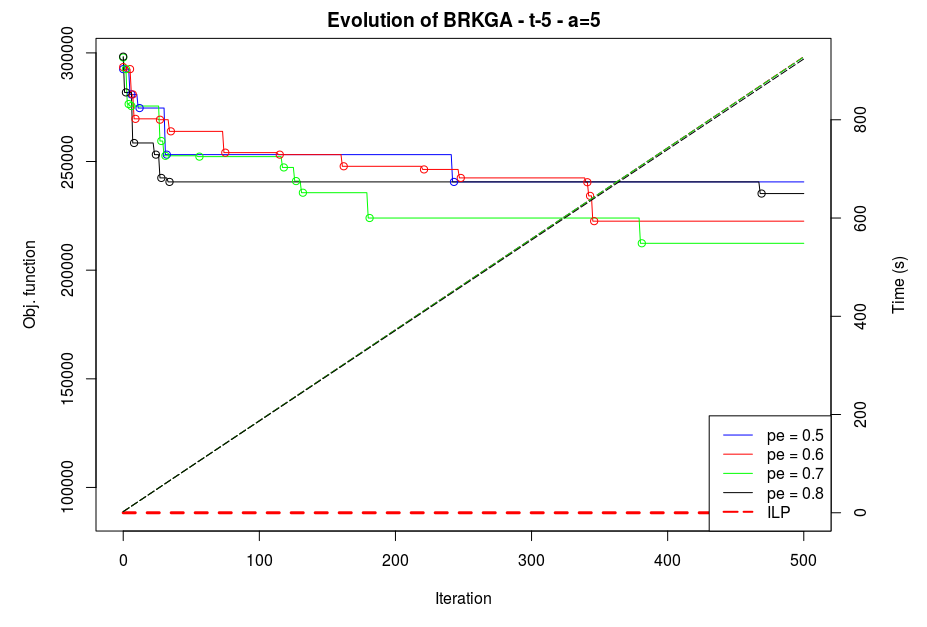
\includegraphics[scale=0.245]{metaheuristics/BRKGA-miquel-tubau-5--5}
        \centeredcaption{Illustration of the trace for the input \textit{t-5}.
        $a = 5$, $p=250$, $p_e=43$, $p_m=50$.}
        \label{fig:trace:brkga:t-5:5}
    \end{subfigure}
    \begin{subfigure}{0.45\textwidth}
        \centering
        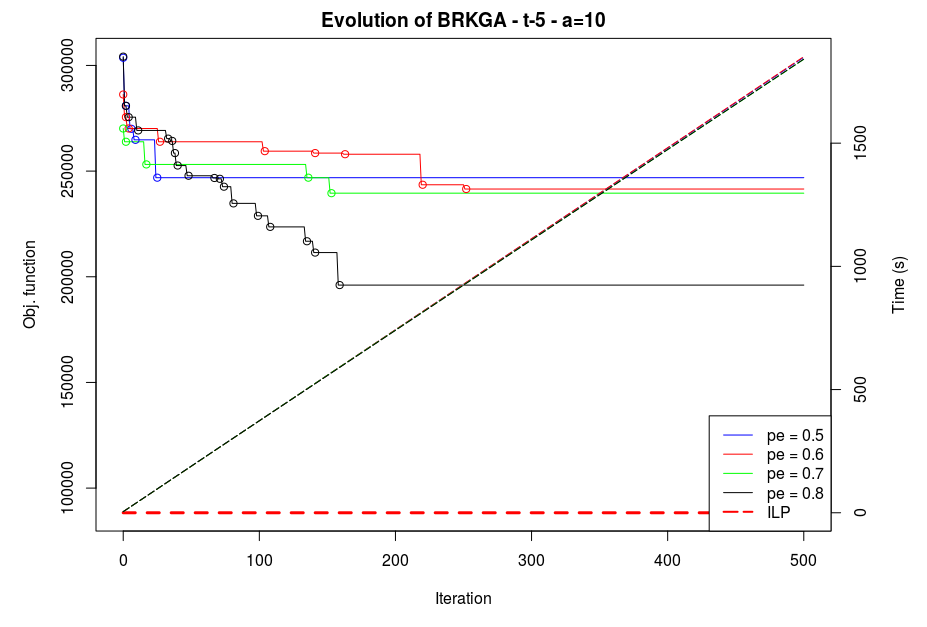
\includegraphics[scale=0.245]{metaheuristics/BRKGA-miquel-tubau-5--10}
        \centeredcaption{Illustration of the trace for the input \textit{t-5}.
        $a = 10$, $p=500$, $p_e=87$, $p_m=100$.}
        \label{fig:trace:brkga:t-5:10}
    \end{subfigure}
    \begin{subfigure}{0.45\textwidth}
        \centering
        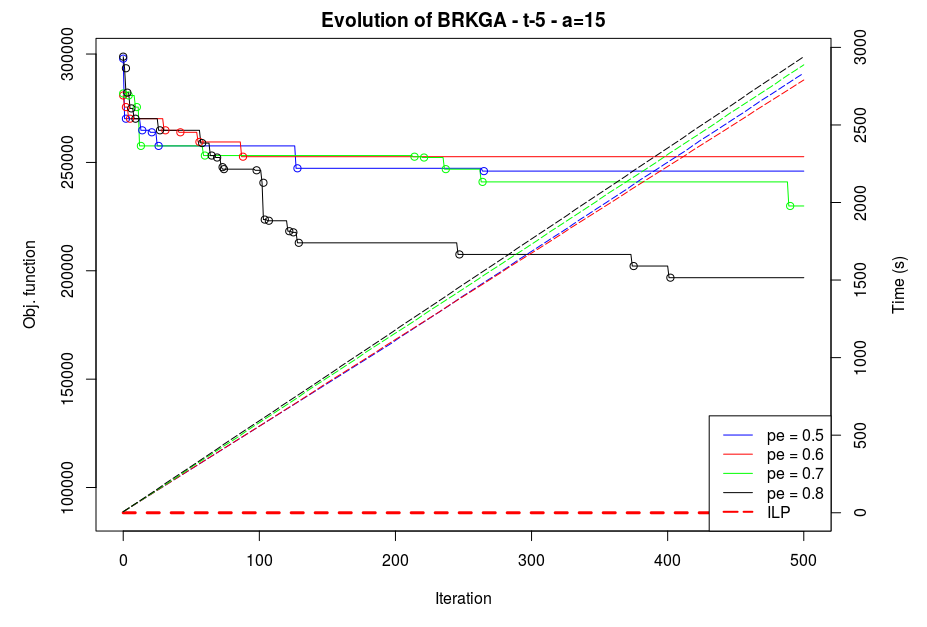
\includegraphics[scale=0.245]{metaheuristics/BRKGA-miquel-tubau-5--15}
        \centeredcaption{Illustration of the trace for the input \textit{t-5}.
        $a = 15$, $p=750$, $p_e=131$, $p_m=250$.}
        \label{fig:trace:brkga:t-5:15}
    \end{subfigure}
    \begin{subfigure}{0.45\textwidth}
        \centering
        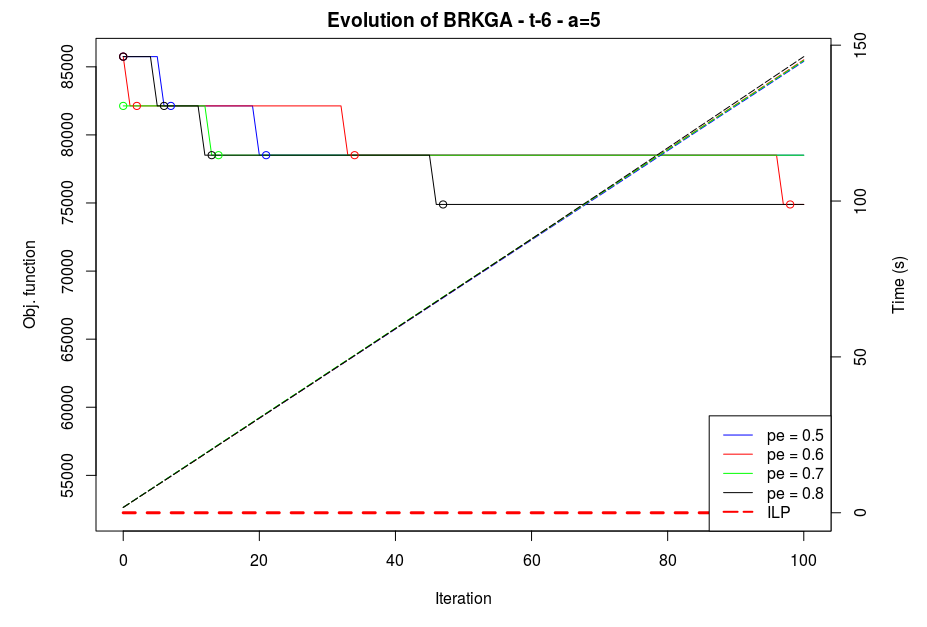
\includegraphics[scale=0.245]{metaheuristics/BRKGA-miquel-tubau-6--5}
        \centeredcaption{Illustration of the trace for the input \textit{t-6}.
        $a = 5$, $p=250$, $p_e=43$, $p_m=50$.}
        \label{fig:trace:brkga:t-6:5}
    \end{subfigure}\\
    \begin{subfigure}{0.45\textwidth}
        \centering
        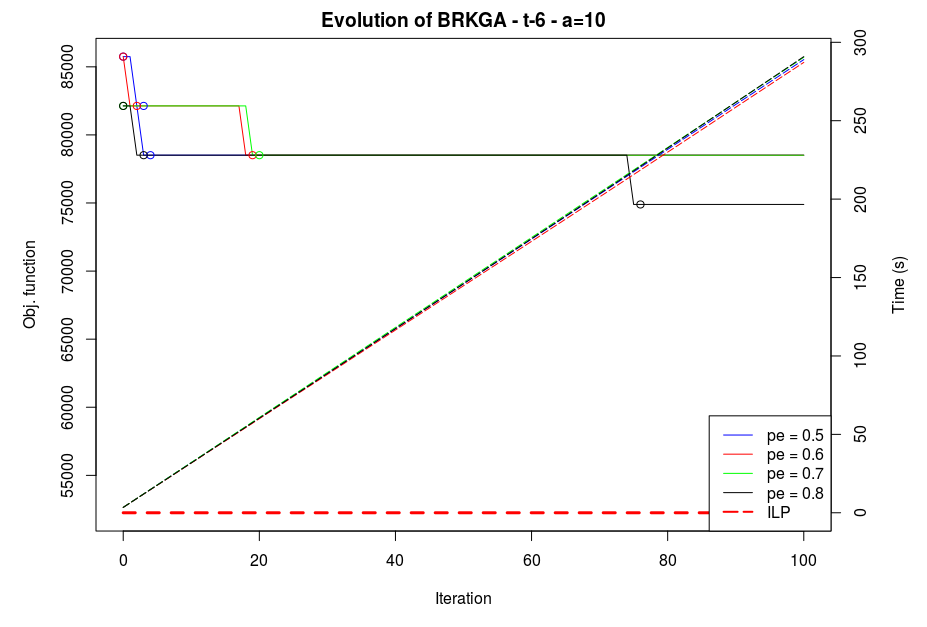
\includegraphics[scale=0.245]{metaheuristics/BRKGA-miquel-tubau-6--10}
        \centeredcaption{Illustration of the trace for the input \textit{t-6}.
        $a = 10$, $p=500$, $p_e=87$, $p_m=100$.}
        \label{fig:trace:brkga:t-6:10}
    \end{subfigure}
    \begin{subfigure}{0.45\textwidth}
        \centering
        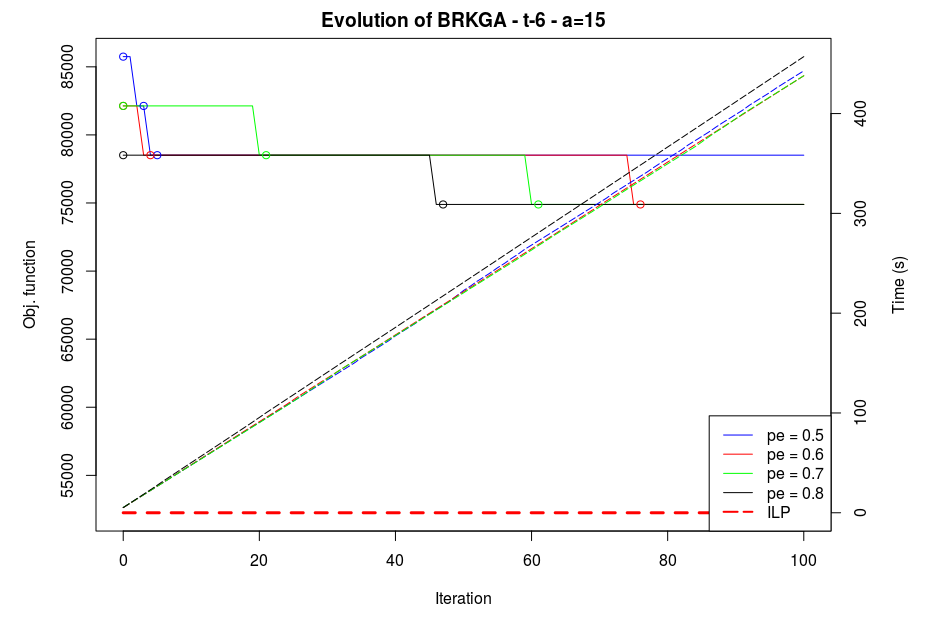
\includegraphics[scale=0.245]{metaheuristics/BRKGA-miquel-tubau-6--15}
        \centeredcaption{Illustration of the trace for the input \textit{t-6}.
        $a = 15$, $p=750$, $p_e=131$, $p_m=250$.}
        \label{fig:trace:brkga:t-6:15}
    \end{subfigure}
    \centeredcaption{Evolution of the BRKGA procedure for the inputs \textit{t-5} and
    \textit{t-6} and values of $a = 5, 10, 15$.}
    \label{fig:trace:brkga:t-5--t-6}
\end{figure}

